\documentclass[12pt,a4paper]{report}

%adjust your page margins here
\usepackage[top=0.70in, bottom=0.70in, left=0.8in,right=0.80in]{geometry} % setting the page alignment with this package
\usepackage[pdftex]{graphicx} %for embedding images
\usepackage{ragged2e}
\usepackage[%dvips, % commented for pdflatex
bookmarks,  colorlinks=false]{hyperref} %for creating links in the pdf version and other additional pdf attributes, no effect on the printed document
\hypersetup{%
    pdfborder = {0 0 0}
}
\usepackage[final]{pdfpages} %for embedding another pdf, remove if not required
\usepackage{float} %used for figure placement with H as a parameter
\usepackage{hyperref}
\usepackage{graphicx}
\usepackage{pslatex} % for times new roman, old package, but works
\usepackage{array} % for making text bold in table
\usepackage{setspace}
\usepackage{float}
\usepackage{enumerate}
\usepackage{longtable}

\usepackage[font=small,labelfont=bf]{caption}
\def\figurename{\textbf{Figure }}
\usepackage{siunitx}
\usepackage{listings}
\usepackage{color}
\usepackage{graphicx}
\graphicspath{{project/images/}}
\definecolor{dkgreen}{rgb}{0,0.6,0}
\definecolor{gray}{rgb}{0.5,0.5,0.5}
\definecolor{mauve}{rgb}{0.58,0,0.82}
 
\lstset{ %
  language=Java,                % the language of the code
  basicstyle=\footnotesize,           % the size of the fonts that are used for the code
  numbers=left,                   % where to put the line-numbers
  numberstyle=\tiny\color{gray},  % the style that is used for the line-numbers
  stepnumber=1,                   % each line is numbered
  numbersep=5pt,                  % how far the line-numbers are from the code
  backgroundcolor=\color{white},      % choose the background color. You must add \usepackage{color}
  showspaces=false,               % show spaces adding particular underscores
  showstringspaces=false,         % underline spaces within strings
  showtabs=false,                 % show tabs within strings adding particular underscores
  frame=single,                   % adds a frame around the code
  rulecolor=\color{black},        % if not set, the frame-color may be changed on line-breaks within not-black text (e.g. commens (green here))
  tabsize=2,                      % sets default tabsize to 2 spaces
  captionpos=b,                   % sets the caption-position to bottom
  breaklines=true,                % sets automatic line breaking
  breakatwhitespace=false,        % sets if automatic breaks should only happen at whitespace
  title=\lstname,                   % show the filename of files included with \lstinputlisting;
                                  % also try caption instead of title
  keywordstyle=\color{blue},          % keyword style
  commentstyle=\color{dkgreen},       % comment style
  stringstyle=\color{mauve},         % string literal style
  escapeinside={\%*}{*)},            % if you want to add a comment within your code
  morekeywords={*,...}               % if you want to add more keywords to the set
}

%For the header and footer
\usepackage{fancyhdr}
\fancypagestyle{plain}{%
\fancyfoot[L]{\emph{ECE Department, PESIT-BSC, Bangalore}} % except the center
\fancyfoot[R]{\thepage}
\renewcommand{\headrulewidth}{0.4pt}
\renewcommand{\footrulewidth}{0.4pt}
}

\pagestyle{fancy}

%\rhead{\emph{NAME OF PROJECT}}

\fancyfoot[LO,LE]{\emph{ECE Department, PESIT-BSC, Bangalore}}
\cfoot{}
\fancyfoot[RO, RE]{\thepage}
\renewcommand{\headrulewidth}{0.4pt}
\renewcommand{\footrulewidth}{0.4pt}
%For the header and footer Over

%Page Border
\usepackage{pgf}
\usepackage{pgfpages}

\pgfpagesdeclarelayout{boxed}
{
  \edef\pgfpageoptionborder{0pt}
}
{
  \pgfpagesphysicalpageoptions
  {%
    logical pages=1,%
  }
  \pgfpageslogicalpageoptions{1}
  {
    border code=\pgfsetlinewidth{2pt}\pgfstroke,%
    border shrink=\pgfpageoptionborder,%
    resized width=.95\pgfphysicalwidth,%
    resized height=.95\pgfphysicalheight,%
    center=\pgfpoint{.5\pgfphysicalwidth}{.5\pgfphysicalheight}%
  }%
}
\pgfpagesuselayout{boxed}
\setlength{\parindent}{1cm}
%GLOBAL SETTINGS OVER, DOCUMENT BEGINS
\begin{document}
\renewcommand\bibname{References}
\lhead{ }

%FROM HERE YOUR PAGES START GETTING ADDED

% includes the cover page
\newpage
\begin{center}
\thispagestyle{empty}
\Large{\textbf{VISVESVARAYA TECHNOLOGICAL UNIVERSITY\\ \large{BELAGAVI - 590018}}}\\
\begin{figure}[h]
	\centering
	
\includegraphics[scale=0.6]{project/images/vtu_new_logo}
	\label{fig:vtulogo}
\end{figure}
\large{\textbf{Project Report\\ on \\}}
\LARGE{\textsc {\textbf{``Remote Controlled Solar Chargeable Patrolling Robot''}}}\\
\large{\textbf{\\Submitted in partial fulfillment of the requirements for the VIII Semester\\}}
\Large{\textbf{\\Bachelor of Engineering \\ in \\ ELECTRONICS AND COMMUNICATION ENGINEERING\\ For the Academic Year \\ 2020-2021}}
\Large{\textbf{\\BY}}\\
\begin{table}[h]
\centering
\Large{
\begin{tabular}{>{\bfseries}lc>{\bfseries}r}
Mayank Saini & & 1PE17EC075\\Rahul Reddy V & & 1PE17EC098\\Rohit Prabhu M & & 1PE17EC105\\Shrishti Upadhyay & & 1PE17EC133\\
\end{tabular}}
\end{table}
\vspace{0.5cm}
\large{\textbf{UNDER THE GUIDANCE OF}}\\
\large{\textbf{Prof. Ananda M}}\\
\large{\textbf{Professor, Dept. of ECE, PESITBSC}}\\
\begin{figure}[h]
	\centering
	
\includegraphics[scale = 0.8]{project/images/pesitbsc_logo}
	\label{fig:pesitbsclogo}
\end{figure}
\Large{\textbf{Department of Electronics and Communication Engineering}}\\
\Large{\textbf{PESIT - BANGALORE SOUTH CAMPUS}}
\large{\textbf{\\Hosur Road, Bengaluru - 560100}}\\
\newpage
\end{center}
\newpage

\definecolor{mygreen}{RGB}{34, 139, 34}
\definecolor{myred}{RGB}{165, 42, 42}
\newpage
\begin{center}
	\thispagestyle{empty}
	\Large{\textbf{\color{myred}VISVESVARAYA TECHNOLOGICAL UNIVERSITY\\ \large{BELAGAVI - 590018}}}\\
	\begin{figure}[h]
		\centering
		
\includegraphics[scale=0.6]{project/images/vtu_new_logo}
		\label{fig:vtulogo}
	\end{figure}
	\large{\textbf{Project Report\\ on \\}}
	\LARGE{\textsc {\textbf{\color{blue}``Remote Controlled Solar Chargeable Patrolling Robot''}}}\\
	\large{\textbf{\\Submitted in partial fulfillment of the requirements for the VIII Semester\\}}
	\Large{\textbf{\\ \color{mygreen}Bachelor of Engineering \\ in \\ ELECTRONICS AND COMMUNICATION ENGINEERING\\ For the Academic Year \\ 2020-2021}}
	\Large{\textbf{\\BY}}\\
	\begin{table}[h]
		\centering
		\Large{
			\begin{tabular}{>{\bfseries}lc>{\bfseries}r}
				Mayank Saini & & 1PE17EC075\\Rahul Reddy V & & 1PE17EC098\\Rohit Prabhu M & & 1PE17EC105\\Shrishti Upadhyay & & 1PE17EC133\\
		\end{tabular}}
	\end{table}
	\vspace{0.5cm}
	\large{\textbf{UNDER THE GUIDANCE OF}}\\ 
	\large{\textbf{\color{mygreen}Prof. Ananda M}}\\
	\large{\textbf{\color{mygreen}Professor, Dept. of ECE, PESIT-BSC}}\\
	\begin{figure}[h]
		\centering
		
\includegraphics[scale = 0.8]{project/images/pesitbsc_logo}
		\label{fig:pesitbsclogo}
	\end{figure}
	\Large{\textbf{Department of Electronics and Communication Engineering}}\\
	\Large{\textbf{PESIT - BANGALORE SOUTH CAMPUS}}
	\large{\textbf{\\Hosur Road, Bengaluru - 560100}}\\
	\newpage
\end{center}
\newpage

% includes the certificate page
\begin{center}
\thispagestyle{empty}

\LARGE{\textbf{PESIT - BANGALORE SOUTH CAMPUS}} 
\large{\textbf{\\ HOSUR ROAD, BENGALURU - 560100}} \\ 
\large{\textbf{DEPARTMENT OF ELECTRONICS AND COMMUNICATION ENGINEERING}}\\[0.5cm]


\includegraphics[scale=1]{project/images/pesitbsc_logo}\\[0.5cm]

{\Large \textbf{CERTIFICATE}}\\[0.5cm]
\end{center}
\linespread{1.13}
\begin{flushleft}
\justify
\large{This is to certify that the project work entitled ``\textbf{Remote Controlled Solar \\Chargeable Patrolling Robot}" carried out by ``\textbf{Mayank Saini, Rahul Reddy V, Rohit Prabhu M, Shrishti Upadhyay} bearing \textbf{1PE17EC075, 1PE17EC098, \\1PE17EC105, 1PE17EC133}" respectively in partial fulfillment for the award of Degree of Bachelors (Bachelors of Engineering) in Electronics and Communication Engineering of Visvesvaraya Technological University, Belagavi during the year 2020-2021. It is certified that all suggestions indicated for internal assessment have been incorporated in the report. The project report has been approved as it satisfies the academic requirements in respect of project work prescribed for the said Degree.}
\end{flushleft}
\begin{spacing}{0}
\vspace{3.0cm}
\large{ Signature of the Guide} \hspace*{0.2in} \large{ Signature of the HOD} \hspace*{0.3in} \large{ Signature of the Principal}\\[0.2cm]

\textbf{Prof. Ananda M}
\hspace*{0.6in}\large{\textbf{Dr. Subhash Kulkarni}}\hspace*{0.4in}\large{\textbf{Dr. Subhash Kulkarni}}\\ [0.2cm]

\textbf{Professor}
\hspace*{1.5in}\textbf{HOD, ECE}\hspace*{1in}\textbf{Principal, PESIT-BSC} \\[1.2cm]

\Large{\textbf{External Viva }}\\[0.5cm]
\large{\hspace*{0.3in}\textbf{Name of the Examiners}} \hspace*{2in} \large{\textbf{Signature with Date}}\\[1cm]
1. \\[1.2cm]
2. \\

\end{spacing} 
\newpage

% includes the acknowledgements page
\begin{center}
\thispagestyle{empty}
\LARGE{\textbf{Acknowledgements}}\\[1cm]
\end{center}
\linespread{1.13}

\begin{large}
We would like to express our sincere gratitude to all the lecturers and staff of the Electronics and Communication department for extending their help and guidance towards our project.
\newline

We would like to thank the college management and express our sincere gratitude to Dr. Subhash Kulkarni, Principal/Head of Department, Electronics and Communication Engineering for having given us the opportunity for the completion of this project.
\newline

We would also like to express our deepest appreciation and gratitude to our project guide Mr. Ananda M, Assistant Professor, for providing us valuable insights throughout our journey. We would like to thank him for all the encouragement and support that was necessary for the progress of this project.
\newline

We would also like to thank our friends who volunteered and helped us with enthusiasm in learning various elements that we used in our project. 
\end{large} 
\newpage

\begin{center}
\thispagestyle{empty}
\vspace{2cm}
\LARGE{\textbf{ABSTRACT}}\\[1.0cm]
\end{center}
\thispagestyle{empty}
\large{\paragraph{}Increasing numbers of crimes around the globe have created a demand for high level of safety and security. At the same time with the fast paced world there has been a requirement to reduce human effort. Many  people are increasingly approaching solutions offered by technology to tackle this.
\newline

Our project aims at introducing a product in the market that not only ensures security of a bounded area , but also focuses on safety and right to privacy by maintaining a highly secure data storage system. Designed and realized in this project, the robot is equipped with a camera, microphone and ultrasonic sensors that  provide remote visuals and audio streams. This is done with the help of a Raspberry Pi and Wi-Fi module. Solar charging of the robot allows conservation of non renewable resources, thus helping us reduce carbon footprint.
}\\
\newline
\textbf{Keywords: }Robot, Camera, Microphone, Ultrasonic sensors, Raspberry Pi, Wi-Fi, Solar Panels. % adds the Research Methodology page
\newpage

%TABLE OF CONTENTS AND LIST OF FIGURES ARE AUTOMATICALLY ADDED BY FOLLOWING COMMANDS
%ADD FIGURE OF TABLES IF YOU NEED TO, CHECK DOCUMENTATION
\pagenumbering{roman} %numbering before main content starts


%To reset the Header & Footer for TOC and LOF
\pagestyle{empty}
\addtocontents{toc}{\protect\thispagestyle{empty}}
\tableofcontents % adds Index Page

\addtocontents{lof}{\protect\thispagestyle{empty}}
\listoffigures % adds List of Figures

\addtocontents{lot}{\protect\thispagestyle{empty}}
%\listoftables

\cleardoublepage

%And reset back the settings we choose for Header and Footer
\pagestyle{fancy}

\newpage
\pagenumbering{arabic} %reset numbering to normal for the main content

\chapter{Introduction}
\section{Objective}
\paragraph{}To reduce human effort whilst maintaining the integrity of a system and at the same time improving the efficiency in applications requiring surveillance or security by providing a movable camera/microphone on a RC controlled robot supported by Wi-Fi.
\section{Problem statement}
\paragraph{}Crimes like Robbery, breaking and entering, threats to ones safety have made all organizations aware and have forced them to take preventive actions to preclude occurrence of such incidents. It is not just governments or organizations that are choosing to wear a defensive posture, but citizens at an individual level as well, are worried about personal, home and organizational security.
\newline

Increasing concerns about business and private property surveillance has given manufacturers and vendors of security equipments a chance to sell these systems by leveraging this fear. Sales figures of security systems are skyrocketing as people tend to believe that these systems can add a layer of security and safeguard their possessions in case of any incident.
\newline

The major problem with the development of these devices are to make them compact and light weight. With respect to the project some major hurdles include dealing with huge amounts of data storage that has to be highly secured to ensure the privacy of the organizational content. Another problem that we face is to establish a method to make controlling of the robot very handy,i.e obtaining a wireless control between the robot and the keyboard.
\section{Problem Solution}
\paragraph{}Our project aims at introducing a similar product in the market that not only ensures security of a bounded area , but also focuses on safety and right to privacy by maintaining a highly secure data storage system.
\newline

The primary objective of our product is to provide remote surveillance to enhance security in an organization. it can be used to monitor inaccessible areas henceforth reducing the risk to human lives.
\newline

The robot can be used to increase efficiency of observation and data accumulation in-case of repetitive and tedious tasks. In short, the robot provides remotely accessible and monitored visuals and audio streams to increase the efficiency of security and surveillance while reducing human effort and maintaining safe cloud storage of data.
\newline

The solar charging allows conservation of non renewable resources, thus helping us reduce carbon footprint. This product is environment friendly and is a step towards sustainable development.
 % adds the introduction page
\chapter{Literature Survey}
\section{Overview}
\paragraph{}The literature survey of a project forms it's backbone, it defines the path and approach to a project. This formed the base of our project that we referred to whenever needed and looked upon it for guidance.
\newline

We started our literature survey by watching many videos on YouTube, videos of remote controlled robot, various types of robot structuring. After watching tons of these videos we studied about various microprocessors that would form the core of our project. We tried to build upon an communication algorithm between our robot and other components.
\newline

We referred to various IEEE papers for similar projects and took inspiration.After long hours of thorough research and study we decided on major segments of our projects. The two segments that we have completed working on are the web application for live feed and the remote control of the robot using keyboard.

\section{Web Application Development}
\paragraph{}In this study via an IEEE paper, a web application was presented to be interface for all the
functionality we intended to provide, live video stream monitoring, motor
control of the robots, authentication of clients, download option for videos
stream etc.
\newline

Since our motor control code was already written in Python, we decided to
make use of python for development of our web application as well by using FLASK. We came across the fact that tens of thousands of web applications are written in Flask, a Python-based web framework, and that this is a standard practice for these kind of projects.
\newline 

There is a rich ecosystem of extensions available in flask. In another IEEE paper, we studied about how to use Flask python module for web application and OpenCV for streaming the video feed from the robot camera.
\newline

We already were capable to design and code HTML and CSS files for web application and code python script for motor control and video streaming.Finally we learnt Flask framework by watching a YouTube video tutorial.

\section{Remote Control of Robot}
\paragraph{}Obtaining wireless control between the robot and the keyboard was one of the main obstacles of the project. Since we are using the ‘a’, ’w’, ‘s’ and ‘d’ keys to control the movement of the robot we had to make sure that the delay between the moments when the key was pressed and the data being received by the robot was less in order to make it a real time embedded system. Hence, we had to choose an appropriate data transfer protocol to meet these requirements. Upon doing research we have decided to use a local area network (LAN) and have also decided to choose TCP/IP sockets as the mode of communication due to its fast nature of data transfer and also due to its peer-to-peer connection.
\newline

The heart of the robot is the raspberry pi 4 (2 GB RAM). After a lot of study we have chosen to use Raspberry Pi over the conventional micro-controllers like Arduino or ESP8266 and the reasons are as follows:
\begin{enumerate}[a. ]
 \item The Raspberry Pi being a microprocessor has a real time OS whose kernel is responsible for handling applications and can thus be used to run multiple \\applications at the same time and hence multithreading need not be introduced in the application code.
 \item The Raspberry Pi has inbuilt Wi-Fi and Bluetooth modules and thus doesn't need separate modules for the same. No additional code is required to connect to the Wi-Fi.
 \item The Raspberry Pi has 4 USB ports and can thus support USB devices like \\microphone and cameras.
 \item The Raspberry Pi also has an inbuilt camera slot where we can attach the \\Pi-Camera for streaming live feed.
 \item The Raspberry pi has 40 GPIO headers out of which 4 are available as PWM pins and can thus be used to control the speed of the motors.
 \item The Raspberry Pi GPIOs can be accessed and controlled using python code.
\end{enumerate}
The OS run on the raspberry pi is Raspbian OS. The reasons why we have used the OS are as follows:
\begin{enumerate}[a. ]
 \item Raspbian is version of Debian used for the Raspberry Pi. Hence it is very secure.
 \item VNC server is inbuilt and freely available on Raspbian and thus there is no need of a separate monitor nor is there any need to install it again. 
 \item Package installations in Raspbian are simple as installations can be done by running Linux commands in the terminal.
\end{enumerate}

Choosing a camera for viewing live feed was also another important task. After surfing the web for various cameras we finally decided to use the raspberry pi camera v2.1. The reason why we used it is because it’s a camera specially meant to be used on the Raspberry Pi and thus has good amount of support to start live streams and capture videos and pictures.
\newpage % adds the Literature Survey page
\chapter{Hardware and Software Requirements Specification}
\section{Hardware Specification}
\subsection{Raspberry Pi 4}
\paragraph{} Raspberry Pi microprocessor is most preferred when developing advanced \\applications. Raspberry Pi is an open source platform where one can get a lot of related information so you can customize the system depending on the need. 
\subsubsection*{Features of Raspberry Pi 4}
\begin{enumerate}
\item Broadcom BCM2711, Quad core Cortex-A72 (ARM v8) 64-bit SoC @ 1.5GHz
\item 2GB, 4GB or 8GB LPDDR4-3200 SDRAM (depending on model)
\item 2.4 GHz and 5.0 GHz IEEE 802.11ac wireless, Bluetooth 5.0, BLE
\item Gigabit Ethernet
\item 2 USB 3.0 ports; 2 USB 2.0 ports.
\item Raspberry Pi standard 40 pin GPIO header (fully backwards compatible with previous boards)
\item 2 × micro-HDMI ports (up to 4kp60 supported)
\item 2-lane MIPI DSI display port
\item 2-lane MIPI CSI camera port
\item 4-pole stereo audio and composite video port
\item H.265 (4kp60 decode), H264 (1080p60 decode, 1080p30 encode)
\item OpenGL ES 3.0 graphics
\item Micro-SD card slot for loading operating system and data storage
\item 5V DC via USB-C connector (minimum 3A*)
\item 5V DC via GPIO header (minimum 3A*)
\item Power over Ethernet (PoE) enabled (requires separate PoE HAT)
\item Operating temperature: \ang{0}C – \ang{50}C ambient
\end{enumerate}
* A good quality 2.5A power supply can be used if downstream USB peripherals consume less than 500mA in total.\\
\begin{figure}[h]
\centering
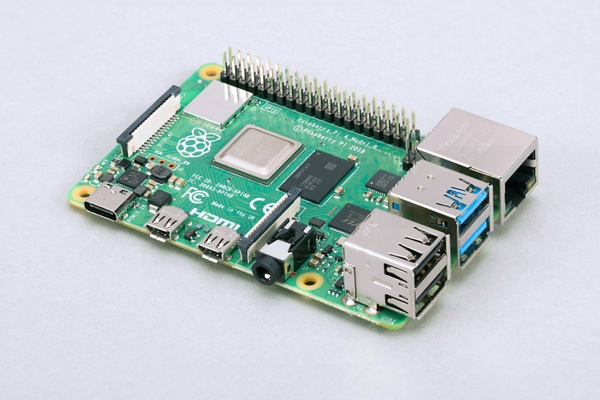
\includegraphics[scale=0.5]{rpi.jpg}
\caption{Raspberry Pi 4} \vspace{1cm}
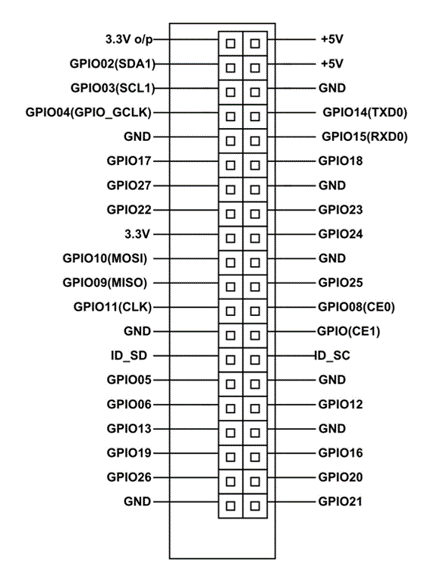
\includegraphics[scale=0.5]{rpipin.png}
\caption{Raspberry Pi Pin-out}
\end{figure}
\subsection{Raspberry Pi Camera}
The Raspberry Pi Camera Modules are official products from the Raspberry Pi \\Foundation. The original 5-megapixel model was released in 2013, and an 8-megapixel Camera Module v2 was released in 2016. For both iterations, there are visible light and infrared versions. A 12-megapixel High Quality Camera was released in 2020.
\begin{figure}[h]
\centering
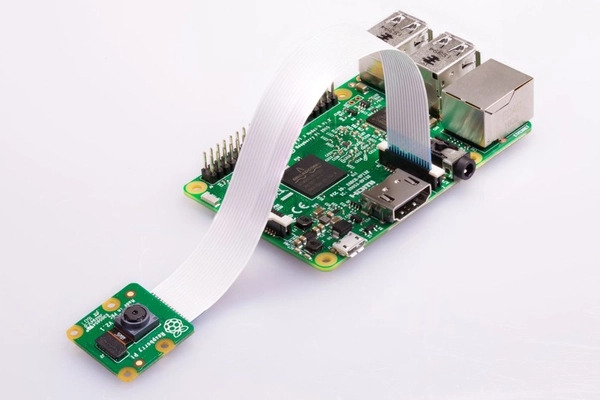
\includegraphics[scale=0.5]{rpicam.jpg}
\caption{Raspberry Pi Camera v2.1}
\end{figure}
\subsection{Motors and its Drivers}
L298N Motor Driver Module is a high power motor driver module for driving DC and Stepper Motors. This module consists of an L298 motor driver IC and a 78M05 5V regulator. L298N Module can control up to 4 DC motors, or 2 DC motors with directional and speed control.
\begin{figure}[h]
\centering
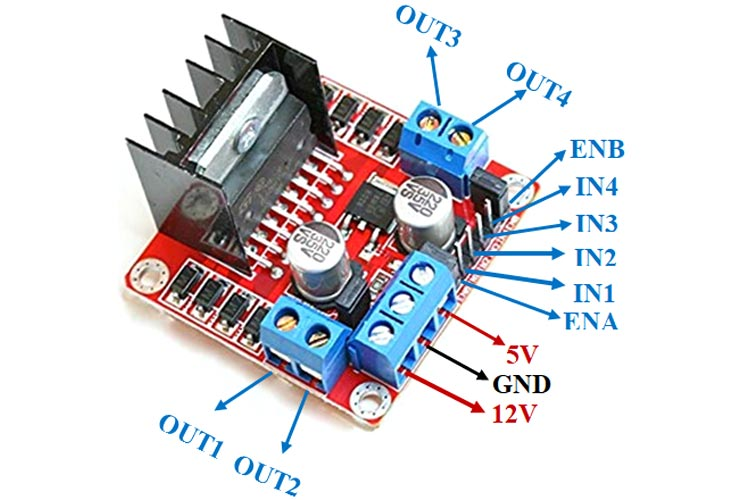
\includegraphics[scale=0.4]{L298N.jpg}
\caption{L298N Motor Driver}
\end{figure}
\subsubsection*{L298N Module Features \& Specifications:}
\begin{enumerate}
\item Driver Model: L298N 2A 
\item Driver Chip: Double H Bridge L298N 
\item Motor Supply Voltage (Maximum): 46V 
\item Motor Supply Current (Maximum): 2A 
\item Logic Voltage: 5V 
\item Driver Voltage: 5-35V 
\item Driver Current:2A 
\item Logical Current:0-36mA 
\item Maximum Power (W): 25W 
\item Heatsink for better performance 
\end{enumerate}

\subsection{LiPo Battery}
A lithium polymer battery, or more correctly lithium-ion polymer battery, is a rechargeable battery of lithium-ion technology using a polymer electrolyte instead of a liquid electrolyte. High conductivity semisolid (gel) polymers form this \\electrolyte. These batteries provide higher specific energy than other lithium battery types and are used in applications where weight is a critical feature, such as mobile devices, radio-controlled aircraft and some electric vehicles 
\begin{figure}[h]
\centering
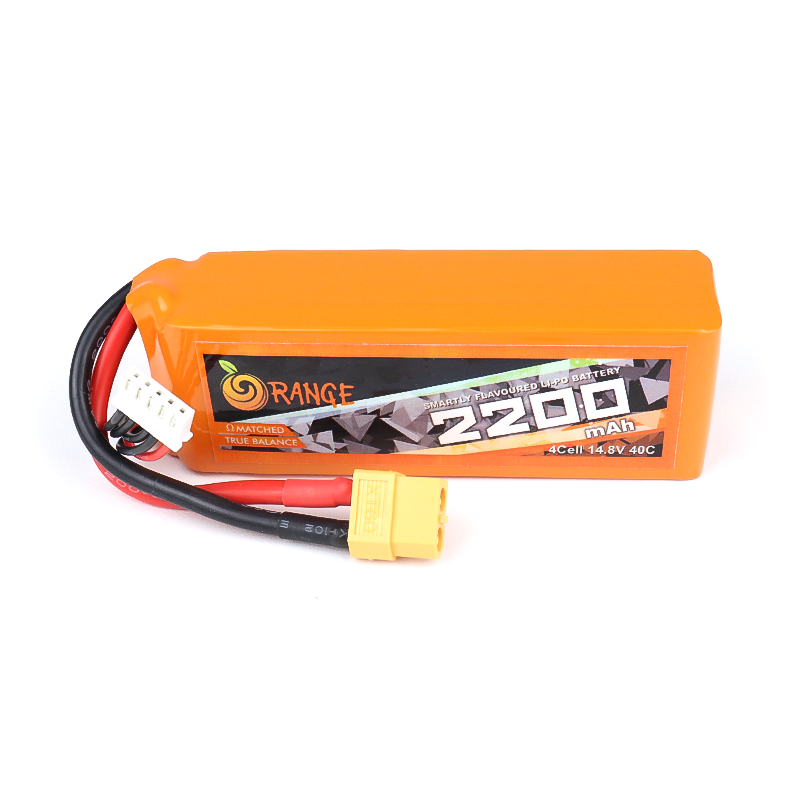
\includegraphics[scale=0.25]{lipo.png}
\caption{LiPo Battery}
\end{figure}
\subsection{Router(Gateway)}
\begin{enumerate}
\item The router is a physical or virtual inter-networking device that is designed to receive, analyze, and forward data packets between computer networks. A router examines a destination IP address of a given data packet, and it uses the headers and forwarding tables to decide the best way to transfer the packets. 
Some important points of routers are given below: 
\item A router is used in LAN (Local Area Network) and WAN (Wide Area Network) environments. For example, it is used in offices for connectivity, and you can also establish the connection between distant networks. 
\item It shares information with other routers in networking. 
\item It uses the routing protocol to transfer the data across a network. 
\end{enumerate}
\begin{figure}[h]
\centering
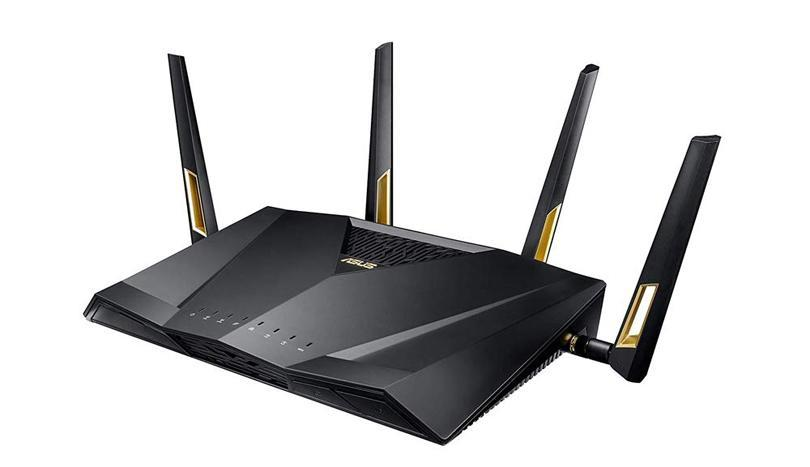
\includegraphics[scale=0.3]{router.jpg}
\caption{Router}
\end{figure}
\section{Software Requirements}
\subsection{Raspbian}
\begin{enumerate}
\item Raspberry Pi OS (formerly Raspbian) is a Debian-based operating system for Raspberry Pi. Since 2015 it has been officially provided by the Raspberry Pi Foundation as the primary operating system for the Raspberry Pi family of compact single-board computers. 
\item Previous Pi OS versions have been 32bit and based on Raspbian core, taking the name Raspbian. Since recent 64bit versions no longer use the Raspbian core, the name has been changed to Raspberry Pi OS for both 64bit and 32bit versions.
\item Raspberry Pi OS is highly optimized for the Raspberry Pi line of compact single-board computers with ARM CPUs. Raspberry Pi OS uses a modified LXDE as its desktop environment with the Openbox stacking window \\manager. 
\end{enumerate}
\begin{figure}[h]
\centering

\includegraphics[scale=0.3]{raspbian.png}
\caption{Rasbian}
\end{figure}
\subsection{Python}
\begin{enumerate}
\item Python is an interpreted, high-level and general-purpose programming \\language. Python's design philosophy emphasizes code readability with its \\notable use of significant whitespace. Its language constructs and object-oriented approach aim to help programmers write clear, logical code for small and \\large-scale projects.
\item Python is dynamically typed and garbage-collected. It supports multiple \\programming paradigms, including structured (particularly, procedural), \\object-oriented and functional programming. Python is often described as a "batteries included" language due to its comprehensive standard library.
\end{enumerate}
\begin{figure}[h]
\centering

\includegraphics[scale=0.3]{python.png}
\caption{Python}
\end{figure}
\newpage
\subsection{Flask}
Flask is a micro web framework written in Python. It is classified as a \\microframework because it does not require particular tools or libraries. It has no database abstraction layer, form validation, or any other components where \\pre-existing third-party libraries provide common functions. However, Flask \\supports extensions that can add application features as if they were implemented in Flask itself. Extensions exist for object-relational mappers, form validation, upload handling, various open authentication technologies and several common framework related tools.
\begin{figure}[h]
\centering

\includegraphics[scale=0.3]{flask.png}
\caption{Flask}
\end{figure}
\chapter{System Design}
\section{Overview}
\paragraph{} This chapter describes the overall design of the wireless communicated robot movement and the web application working for the live feed from camera mounted on the robot. As we already know the hardware and software components used we will further go ahead and discuss the system design that we developed.
\section{Designing the Web Application}
\paragraph{}Web technologies we are using for the project are HTML, CSS, Bootstrap, Python and Flask. These technologies are needed to configured in a proper manner for the web application to work properly. In the directory where the project folder for the web application is established all the constituent files and folders have to be kept in a specific format as supported by Flask.

\begin{figure}[h]
\centering
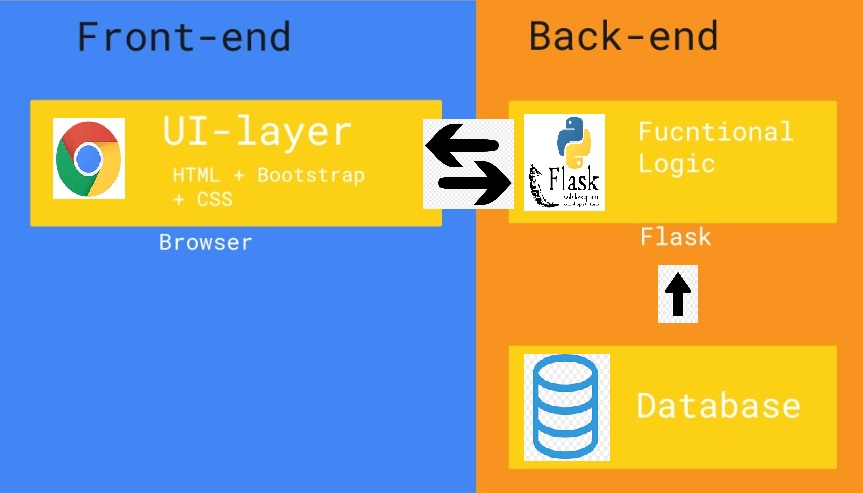
\includegraphics[scale=0.4]{bdweb.jpg}
\caption{Block Diagram of Web Application}
\end{figure}

\subsubsection*{Here is the basic file structure for flask:} 
\texttt{\textbf{\small{yourapp/}}}

\texttt{\small{.py}}

\textbf{\texttt{\small{static/}}}

\hspace{0.5in}\texttt{\small{.js}}

\hspace{0.5in}\texttt{\small{.css}}

\hspace{0.5in}\texttt{\small{Images}}

\textbf{\texttt{\small{templates/}}}

\hspace{0.5in}\texttt{\small{.html}}

\subsubsection*{Description of files:}
\textbf{.py}: contains the actual python code that will import the app
and start the \\development server.\\
\textbf{static/} : contains static files i.e. CSS (including bootstrap), JavaScript, images.\\
\textbf{templates/} : This is where you store your HTML templates
i.e. index.html, \\layout.html\\
Python modules used in app.py (main web app Script/Program):
\begin{enumerate}[1.]
\item Flask - Web application framework
\item CV2 - Library to help the drawing process with Open-CV
\item Sockets - provides access to the BSD socket interface
\item Keyboard - provides various keys-related functions
\item Time - provides various time-related functions
\item Rpi.GPIO - This package provides a class to control the GPIO on a Raspberry Pi.
\end{enumerate}

\section{Designing the remote controlled robot movement}
The heart of the robot is a raspberry pi 4(2GB RAM) which is a credit card sized computer used in a wide range of applications varying from a simple personal \\computer to advanced robotics.  The raspberry pi has an inbuilt Wi-Fi module which can connect to any network. The OS of the raspberry pi resides within an SD card of size 32 GB. The motors of the robot are controlled using the PWM pins available on the 40 pin GPIOS of the raspberry pi. The raspberry pi GPIO pins output a \\current insufficient to drive the motors and hence we have used the L298N motor driver which amplifies the current so that it drives the motors easily. In order to get \\information about the surroundings of the area in which the robot is patrolling we have used three sensors. They are ultrasonic sensors, Picamera v2.1 and a USB mic. The ultrasonic sensor is used to measure distances on all sides of the robot in order to ensure that the robot doesn’t collide with any obstacles in its vicinity. The Picamera acts as the eyes of the robot. The robot is steered using the ‘a’, ’w’, ‘s’ and ‘d’ keys of the robot based on the camera feed received. The USB mic acts like the ears of the robot. Using the mic, the robot can capture audio within its vicinity.
\begin{figure}[h]
\centering
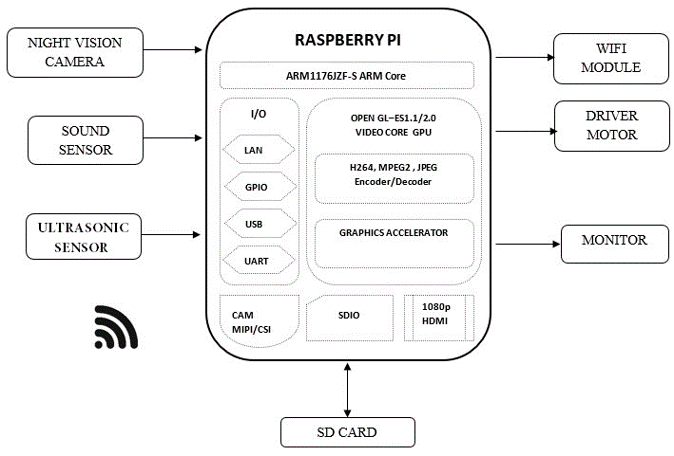
\includegraphics[scale=0.8]{bdrobot.png}
\caption{Block Diagram of Robot}
\end{figure}
\subsection{TCP/IP Communication}
The communication protocol which we have opted to use in our project is the TCP/IP socket protocol.  The TCP/IP socket protocol establishes a peer-to-peer connection between the server and the client followed by which data is transferred in the form of packets of fixed length. In our case each packet is 1024 bytes in length. A socket is one end of a 2-way communication. A socket consists of an IPV4 address and a port number. The connection between the server and the client happens with a series of events occurring on both the server and the client sides.
\subsubsection*{The following occurs on the server side:} 
\begin{enumerate}[1.]
\item Declaration of the socket object: first a socket object is created which is an \\instance of the socket class.
\item Socket binding: The process of assigning a port number to a socket is called socket binding.  
\item Listening for connections: Once the socket has been binded it soon starts listening for connection requests from active clients. 
\item Accepting Client connections: The server accepts all the client connections who are willing to connect to the server. Upon connection the server receives \\connection objects using which the server sends data to the client.
\item Data transfer: The server uses the connection objects to send data to the client.
\end{enumerate}
\subsubsection*{The following occurs on the client side:}
\begin{enumerate}[1.]
\item Declaration of the socket object: first a socket object is created which is an \\instance of the socket class.
\item Connection: The client sends a connection request to the server using the ip and port number of the server. 
\item Data transfer: Once the server accepts the connection of the client, the client starts receiving the data sent by the server.
\end{enumerate}
\subsection{GIX algorithm}
The GIX algorithm is an acronym for “Gone in exchange” Algorithm . The GIX algorithm ensures that data is transferred securely over the internet by using \\encryption and decryption algorithms on the sender and the receiver sides \\respectively.
\subsubsection*{The following occurs on the sender side: }
\begin{enumerate}
\item First the pure control message is received. Which in our case is the key pressed.
\item A random key is chosen and the control message is encrypted using the key.
\item The random key is hidden within the encrypted control message and the final encrypted message is returned.
\item The encrypted message is sent over the internet.
\end{enumerate}
\subsubsection*{The following occurs on the receiver side: }
\begin{enumerate}
\item The encrypted control message is received. 
\item The hidden key is found within the encrypted message.
\item Using the key, the message is decrypted to get the pure control message.
\item Appropriate tasks are performed based on the control message received. 
\end{enumerate}
\begin{figure}[h]
\centering
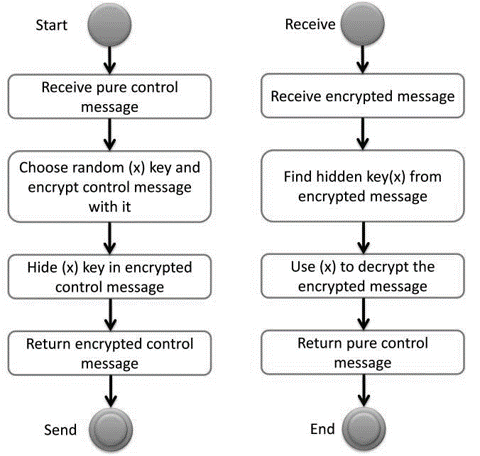
\includegraphics[scale=0.8]{gix.png}
\caption{GIX Algorithm}
\end{figure}

\chapter{Implementation}
\section{Implementation of Website}
To host the live streaming server we make use of a python script in the back-end, communicating with the rendered front-end on the client side. In the script we make use of Open-CV Python Library for streaming and control of the stream parameters. The website contains two main elements which are, Video streaming and Alerts from ultrasonic sensors on the Left, Right and Rear Ends of the Robot. 
\subsection*{Video Streaming}
Video frames are captured by Raspberry Pi Camera which are then converted to JPEG images. These JPEG images are displayed continuously on the website at a high speed. This results in the images appearing to be a Real Time Video.
\subsection*{Ultrasonic Sensor Alerting}
\begin{figure}[h!]
\centering
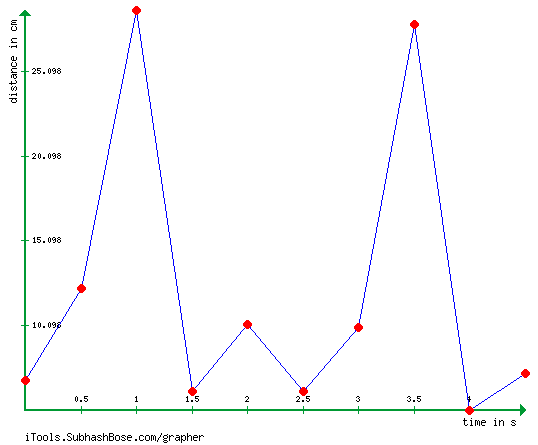
\includegraphics[scale=0.35]{Distance_Graph.png}
\caption{Ultrasonic Distance Graph}
\end{figure}
In Ultrasonic Sensor Alerting, we host an API i.e., host the sensor data acquisition code on a flask server. We make use of JavaScript to request sensor data from the API. Once the Ultrasonic Sensor readings are received, the data is then extracted and is in the JSON format. The data here being the distance.  We then make use of DOM manipulation to trigger alerts on the website application if the distance is less than 10cm.
The above figure represents the distance recorded in Real Time.

\section{Implementation of Robot Movement}
First the keystrokes are recorded using keyboard module in the form of a character,
the recorded characters are then sent from server to client using TCP/IP sockets.
Upon receiving the character on the receiver side the appropriate action is
implemented using an if-else ladder which is reflected by the motion of the robot.
Raspberry Pi GPIO used in Board mode and is connected to the motor driver in the format given below:
\begin{enumerate}[ ]
\item Pin 18 – IN1(Right)
\item Pin 16 – IN2(Right)
\item Pin 15 – IN3(Left)
\item Pin 13 – IN4(Left)
\item Pin 12 – ENA(PWM - Right)
\item Pin 33 – ENB(PWM - Left)
\end{enumerate}
\begin{figure}[h]
\centering
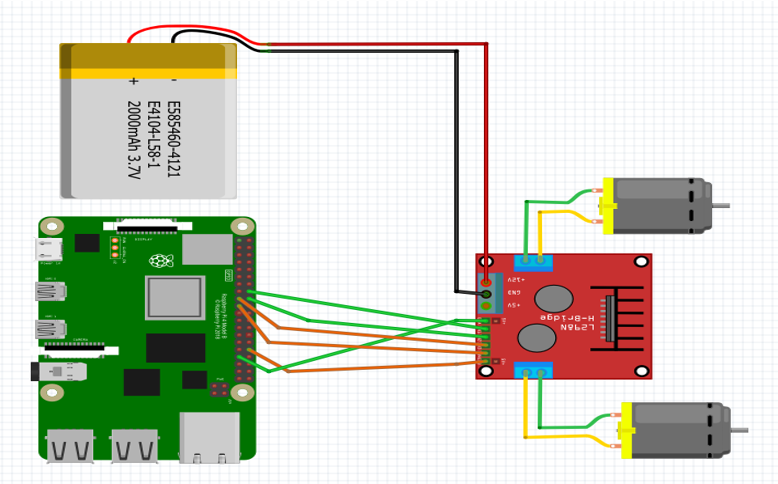
\includegraphics[scale=0.6]{ckt.png}
\caption{Motor Circuit Connections}
\end{figure} % adds the Project Design
\chapter{Result Analysis}
\section{Robot Movement}
The robot movement in various directions was performed by pressing the a, w, s, d keys on the keyboard. The robot reacted spontaneously. This was accomplished with the help of wifi and delay less transfer  of data. Upon pressing of the keys the respective robot movement in different directions was observed. In addition to this we demonstrated the working of the motors by the means of LED bulb s and a table to showed the multidirectional movement.
\begin{figure}[h]
\centering
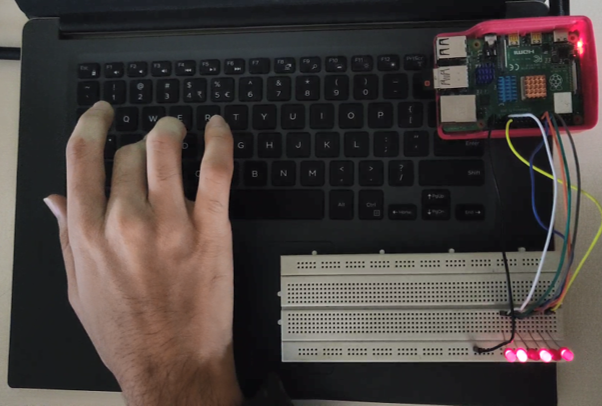
\includegraphics[scale=0.8]{led.png}
\caption{Working of motor using LEDs}
\end{figure}
\newpage
\section{Live Feed Capture}
The camera connected to the raspberry pi gave instant camera feed without any delay. This was reflected on the websites that we developed .It was observed that the camera quality was good and hence clear images were obtained.
\begin{figure}[h]
\centering
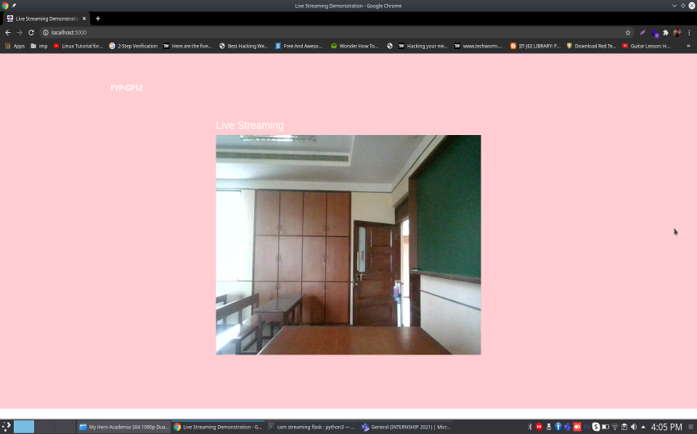
\includegraphics[scale=0.8]{webpage.png}
\caption{Local Live feed on Webpage}
\end{figure}
\chapter{Conclusion and Future Scope}
\section{Conclusion}
\paragraph{}After successfully testing the various segments of our project so far we can conclude that this product can be a very ideal device for surveillance in bounded areas. the robot responds to all the keys in ideal time frame and moves accordingly in different directions. The accuracy of these movements make it a very idealistic equipment.

The live feed capturing from the camera resent on the robot is also very accurate and has minimal or no delay at all. The clarity of the same is astonishing.\\
\newline
After testing and analysing the project so far these are the advantages that we can conclude upon:
\begin{enumerate}
\item Low cost
\item Wireless system makes it compact
\item Easily portable
\item System operates at near real time
\item Makes remote controlling very easy
\item Huge add-ons like obstacle avoidance is possible
\item Eliminates human error
\item Nature friendly as it uses solar charging
\item Ensures data privacy of the user
\end{enumerate}

\section{Future Scope}
\paragraph{}The project that we have implemented has immense future prospective and an abysmal scope for future enhancements. There are limitless possibilities of its usage in the industry. However our main aim was to implement a low cost compact handy remote controlled robot due to which the choices we had for implementation were limited and narrowed down only to a few.\\
\newline
Future applications of the product are as follows:
\begin{enumerate}
\item \textbf{Security management systems}: The robot can be used for patrolling in campuses of various organizations spread over an area. The camera and microphone present on it can provide access to live feed of any corner of the campus at any given point of time. A server setup in the security room can store data in a safe and secure manner.

\item \textbf{Wildlife photography and videography}: The robot can be used by a wildlife photography team in order to observe the flora and fauna for endless hours . As the robot can manage obstacles, it is easier for it to move around in rough terrains . This helps the organization to study the wildlife without disturbing it with human presence. Example mine caves.

\item \textbf{Survey of underground tunnels}: the product can be applicable for uses in data logging and observational surveys that need to be conducted in inaccessible places. For example a survey of underground metro lines or sewage tunnels.

\item \textbf{Information gathering}: The device can be excellent for active reconnaissance. Military observation of a region to locate an enemy or ascertain strategic features. the safe and secure data storage assures national security.
\end{enumerate} % adds the Scheduling and Planning page
\addcontentsline{toc}{chapter}{References}
\begin{thebibliography}{99}
\bibitem{IEEE Paper}
J. Bae, D. Lee and K. Cho, "Speed and Direction Control of Two In-wheel BLDC Motors for the Self-Driving Surveillance Robot," 2020 6th International Conference on Mechatronics and Robotics Engineering (ICMRE), 2020, pp. 17-21, doi: 10.1109/ICMRE49073.2020.9065011.

\bibitem{IEEE Paper}
M. Hamza, M. Atique-ur-Rehman, H. Shafqat and S. B. Khalid, "CGI SCRIPT AND MJPG VIDEO STREAMER BASED SURVEILLANCE ROBOT USING RASPBERRY PI," 2019 16th International Bhurban Conference on Applied Sciences and Technology (IBCAST), 2019, pp. 947-951, doi: 10.1109/IBCAST.2019.8667217.

\bibitem{IEEE Paper} 
A. U. Bokade and V. R. Ratnaparkhe, "Video surveillance robot control using smartphone and Raspberry Pi," 2016 International Conference on Communication and Signal Processing (ICCSP), 2016, pp. 2094-2097, doi: 10.1109/ICCSP.2016.7754547.

\bibitem{IEEE Paper} 
H. R. and M. H. Safwat Hussain, "Surveillance Robot Using Raspberry Pi and IoT," 2018 International Conference on Design Innovations for 3Cs Compute Communicate Control (ICDI3C), 2018, pp. 46-51, doi: 10.1109/ICDI3C.2018.00018.

\bibitem{IEEE Paper} 
M. F. Alvi, F. Junejo, M. W. Baloch and A. J. Rajput, "RoboCop; A Robust Surveillance Robot," 2018 1st International Conference on Advanced Research in Engineering Sciences (ARES), 2018, pp. 1-8, doi: 10.1109/ARESX.2018.8723270.

\bibitem{IEEE Paper} 
S. Meghana, T. V. Nikhil, R. Murali, S. Sanjana, R. Vidhya and K. J. Mohammed, "Design and implementation of surveillance robot for outdoor security," 2017 2nd IEEE International Conference on Recent Trends in Electronics, Information \& Communication Technology (RTEICT), 2017, pp. 1679-1682, doi: 10.1109/RTEICT.2017.8256885.

\bibitem{IEEE Paper} 
N. K. Raghavendra and K. Padmavathi, "Solar Charge Controller for Lithium-Ion Battery," 2018 IEEE International Conference on Power Electronics, Drives and Energy Systems (PEDES), 2018, pp. 1-5, doi: 10.1109/PEDES.2018.8707743.

\bibitem{Website}
Raspberry Pi L298N Interface Tutorial | Control a DC Motor\\
\textit{https://www.electronicshub.org/raspberry-pi-l298n-interface-tutorial-control-dc-motor-l298n-raspberry-pi/}

\bibitem{Website}
Flask For Python3\\
\textit{https://youtu.be/Z1RJmh\_OqeA}

\bibitem{Website}
Solar Battery Charger (LiPo/Li-Ion)\\
\textit{https://youtu.be/kEttqWJrdww}

\bibitem{Website}
Web Basics - Accessing JSON data from URL\\
\textit{https://youtu.be/kIRp6HOQzP8}

\bibitem{Website}
Run a python script forever on Raspberry Pi\\
\textit{https://gist.github.com/skynet-05/f5445b8ad046a08b9469884c12a1a443}

\bibitem{Books}
Raj Kamal, ‖Internet of Things-Architecture and design principles‖, McGraw Hill
Education.

\bibitem{Books}
Holger Karl \& Andreas Willig, "Protocols And Architectures for Wireless Sensor
Networks" , John Wiley, 2005.

\bibitem{Books}
Feng Zhao \& Leonidas J. Guibas, ―Wireless Sensor Networks- An Information
Processing Approach", Elsevier, 2007.
%\bibitem{•} \emph{•} \url{•}
\end{thebibliography}
 % adds the References page
\appendix
\chapter{Review Process}
\section{Phases of Review}
\paragraph{} Project was evaluated at phases with major checkpoints as follows :\\

\textbf {\underline{Pre-Review :  \textit{Defining Problem Statement and Analysis Review} (27/10/2020)}}
\begin{enumerate}
\item Understanding of the problem statement.  
\item Technical understanding of domain. 
\item Identification of differentiating features.
\item Feasibility of conversion to product.
\end{enumerate}

\textbf {\underline{1st Review :  \textit{Literature survey and Project plan Review } (9/11/2020)}}
\begin{enumerate}
\item Clarity in understanding of the problem/project. 
\item Completion of Literature Survey. 
\item Identification of sub-blocks and their interaction.
\item Timeline for completion of project using Gantt chart.
\end{enumerate}

\textbf {\underline{2nd Review :  \textit{Module level design and Test Plan Review} (7/12/2020)}}
\begin{enumerate}
\item Detail design of each module. 
\item Integration and module test plan. 
\item Availability status of required Hardware and Software components.
\item 20\% Completion of Project implementation.
\end{enumerate}
\newpage
    
\textbf {\underline{3rd Review :  \textit{Project Progress Review} (27/5/2021)}}
\begin{enumerate}
\item Adherence to project plan.
\item Completion of module interaction interface design.
\item 50\% Project implementation.
\item Demonstration of completed modules using primitive interfaces 
\end{enumerate}


\textbf {\underline{4th Review :  \textit{Final Demonstration Review} (17/7/2021)}}
\begin{enumerate}
\item 100\% Module implementation and Integration.
\item Quality of packaged full demo presentation.
\item Quality of documentation made across project.
\item Group presentation / communication skill. 
\end{enumerate}




%\appendix
\chapter{Project Planning}
\section{SECTION 1}
\paragraph{} WRITE HERE.

%%\appendix
\chapter{Work Division}
\section{Work Done in 7th Semester}
\paragraph{} WRITE HERE.


\section{Work Done in 8th Semester}
\paragraph{} WRITE HERE.


\end{document}